\documentclass[11pt]{article}
\usepackage[margin=0.9in]{geometry}
\usepackage{booktabs,graphicx,float,amsmath,xcolor,enumitem}
\usepackage[hidelinks]{hyperref}
\usepackage{titlesec}
\titleformat{\section}{\large\bfseries}{\thesection.}{0.5em}{}
\titlespacing*{\section}{0pt}{8pt}{3pt}
\setlength{\parindent}{0pt}
\setlength{\parskip}{4pt}
\setlist{nosep,leftmargin=1.2em}
\newcommand{\taurct}{\hat\tau^{\,\mathrm{RCT}}}
\newcommand{\taunaive}{\hat\tau^{\,\mathrm{naive}}}

\begin{document}

{\Large\bfseries Weekly Project Progress Report, Week 6: Do City Chiefs Grant More Discretionary Tax Exemptions?}

\vspace{2pt}
\textbf{Name:} Tsu Ning Tsao \quad \textbf{Student Number:} 1012713137

\section*{One-Paragraph Research Summary}
\textbf{Research question.} When neighbourhood chiefs (Local) instead of state agents (Central) collect the property tax, do more properties get exempted, and are the extra exemptions justified by the owner's legal status or are they discretionary favours? Later weeks ask for which households the effect is larger (e.g.\ co-ethnic owners). \textbf{Data.} Replication data of Bal\'an et al.\ (2022): the 2018 property-tax campaign in Kananga, D.R.\ Congo. Neighbourhoods (\texttt{a7}) were randomly assigned to Central (\texttt{tmt}=1) or Local (\texttt{tmt}=2). The unit is the property: the collectors' registration record merged with an independent monitoring survey of the owner. This week's full experimental sample is the 5,645 properties in 202 neighbourhoods with exemption status and owner traits recorded. \textbf{Variables.} Outcome $Y$ = \texttt{exempt} (1 if the collector registered the property as tax-exempt); secondary outcomes split exemptions by stated reason and flag \emph{discretionary} exemptions (reason contradicts the owner's traits: ``elderly'' but owner under 55, the legal threshold, or ``widow'' but owner male). Treatment $D$ = \texttt{local}. Covariates: owner age (the selection variable $S$), female, Luluwa (main tribe), works for the state.

\textbf{Track: RCT.} Two datasets: the full experimental sample and the biased sample built below (seed 1465, Recipe B, $S$ = owner age). Code: \texttt{00\_master/00\_master.py} runs \texttt{01\_preanalysis.py} and \texttt{02\_analysis/02\_week6\_benchmark.py}; outputs are in \texttt{03\_output/week6/}.

\section{The experimental benchmark (full sample)}
\begin{table}[H]\centering\small
\caption{Treatment effect of Local on \texttt{exempt}. Rows 1--2: full experimental sample; rows 3--6: biased sample.}
\begin{tabular}{llccc}
\toprule
Sample & Estimator & $\hat\tau$ & Cluster SE & Bootstrap 95\% CI\\
\midrule
Full & Difference in means & 0.019 &  & [-0.043, 0.084]\\
Full & Regression: Y on D + age, female, Luluwa, state job & 0.031 & 0.026 & [-0.023, 0.087]\\
Biased & Difference in means & 0.219 &  & [0.154, 0.285]\\
Biased & Regression: Y on D + female, Luluwa, state job (no S) & 0.200 & 0.032 & [0.135, 0.262]\\
Biased & Regression: Y on D + S + X (backdoor adjustment) & 0.041 & 0.029 & [-0.014, 0.095]\\
Biased & DoWhy backdoor linear regression & 0.039 & & \\
\bottomrule
\end{tabular}

\par\smallskip\footnotesize Standard errors clustered by neighbourhood. Bootstrap: 500 draws, resampling neighbourhoods (the unit of randomisation), seed 1465.
\end{table}
$\taurct = 0.031$: assigning a neighbourhood to chief collection raises the probability that a property is registered as exempt by 3.1 percentage points, from a Central mean of 31.4\% (cluster SE 0.026, bootstrap CI $[-0.023, 0.087]$, so not significant in this subsample). The difference in means (0.019) is smaller because Central happens to have slightly more female owners; across all 14,381 registered properties the raw difference is 4.7 points.

\begin{table}[H]\centering\small
\caption{Where do the extra exemptions come from? Full experimental sample, regression with covariates.}
\begin{tabular}{lccccc}
\toprule
Outcome (0/1) & Central & Local & $\hat\tau$ & SE & $N$\\
\midrule
Any exemption & 0.314 & 0.333 & 0.031 & 0.026 & 5,645\\
Reason: elderly & 0.139 & 0.187 & 0.048** & 0.022 & 5,645\\
Reason: widow & 0.150 & 0.120 & -0.018 & 0.014 & 5,645\\
Reason: other & 0.025 & 0.026 & 0.001 & 0.007 & 5,645\\
Discretionary (reason contradicts owner traits) & 0.039 & 0.040 & -0.001 & 0.007 & 5,645\\
Enumerator disagrees with collector & 0.049 & 0.062 & 0.013 & 0.009 & 5,644\\
\bottomrule
\end{tabular}

\par\smallskip\footnotesize *** $p<0.01$, ** $p<0.05$, * $p<0.1$; SE clustered by neighbourhood.
\end{table}
The increase comes from elderly exemptions (+4.8 points, $p=0.03$), while widow exemptions do not rise. Discretionary exemptions are 3.9\% of properties in both arms, and among exempt properties the discretionary share is 12.6\% in Central and 11.9\% in Local. So far, chiefs exempt more owners who are in fact old, not more owners who do not qualify.

\section{Build the biased sample}
\textbf{Recipe, parameters, seed.} Recipe B, $\alpha=0$, $\gamma=1$, $S$ = owner age (standardised), seed 1465. A Local property is kept with probability $\Lambda(\gamma S_i)$ and a Central property with $\Lambda(-\gamma S_i)$. The story: outside the experiment, a chief would end up collecting from older, long-settled owners he knows, while state agents reach younger owners. \textbf{Sizes.} Full: 2,761 Central, 2,884 Local. Biased: 1,328 Central, 1,412 Local (2,740 kept).

\begin{table}[H]\centering\small
\caption{Balance of baseline covariates, full vs biased sample ($p$ from a regression on $D$, SE clustered by neighbourhood).}
\begin{tabular}{lcccccc}
\toprule
 & \multicolumn{3}{c}{Full sample} & \multicolumn{3}{c}{Biased sample}\\
\cmidrule(lr){2-4}\cmidrule(lr){5-7}
Covariate & Central & Local & $p$ & Central & Local & $p$\\
\midrule
Owner age (S) & 56.4 & 56.1 & 0.659 & 49.8 & 62.8 & 0.000\\
Owner 55 or older & 0.537 & 0.536 & 0.962 & 0.355 & 0.734 & 0.000\\
Owner female & 0.277 & 0.249 & 0.174 & 0.228 & 0.289 & 0.010\\
Owner Luluwa & 0.771 & 0.805 & 0.286 & 0.754 & 0.808 & 0.118\\
Owner works for state & 0.239 & 0.223 & 0.375 & 0.237 & 0.232 & 0.812\\
$N$ & 2,761 & 2,884 & & 1,328 & 1,412 & \\
\bottomrule
\end{tabular}

\end{table}
In the full sample no covariate differs (all $p\ge0.17$). In the biased sample Local owners are 13 years older (62.8 vs 49.8) and 73\% vs 36\% are 55 or older; the female share also moves, because owners aged 55 or older are more often women (32\% vs 15\%).

\begin{figure}[H]\centering
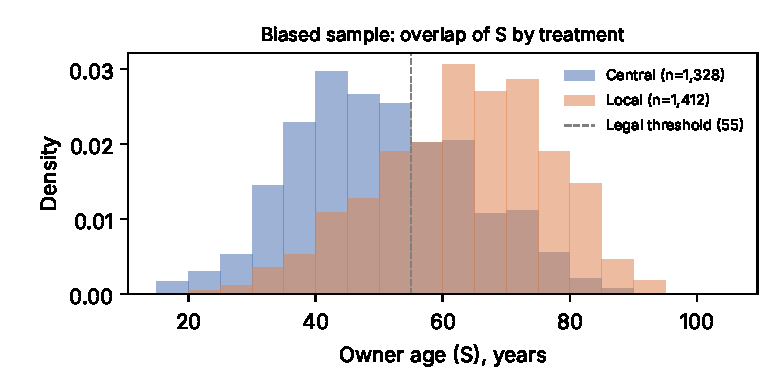
\includegraphics[width=0.62\linewidth]{figure1_overlap.pdf}
\caption{Owner age by treatment, biased sample. Both groups span ages 18 to 88 (Central) and 99 (Local) and share most of the range, so overlap holds.}
\end{figure}

\section{The naive estimate (biased sample)}
On the biased sample the difference in means is 0.219 and the regression of $Y$ on $D$ without $S$ gives $\taunaive = 0.200$ (Table 1, rows 3--4). \textbf{Selecting on owner age changes the estimate from 3.1 to 20.0 percentage points}, because age raises both the chance of being kept in Local and the chance of an (elderly) exemption. Adding $S$ back brings it to 0.041 (row 5).

\section{Test DAG 2 with data (biased sample)}
\begin{figure}[H]\centering
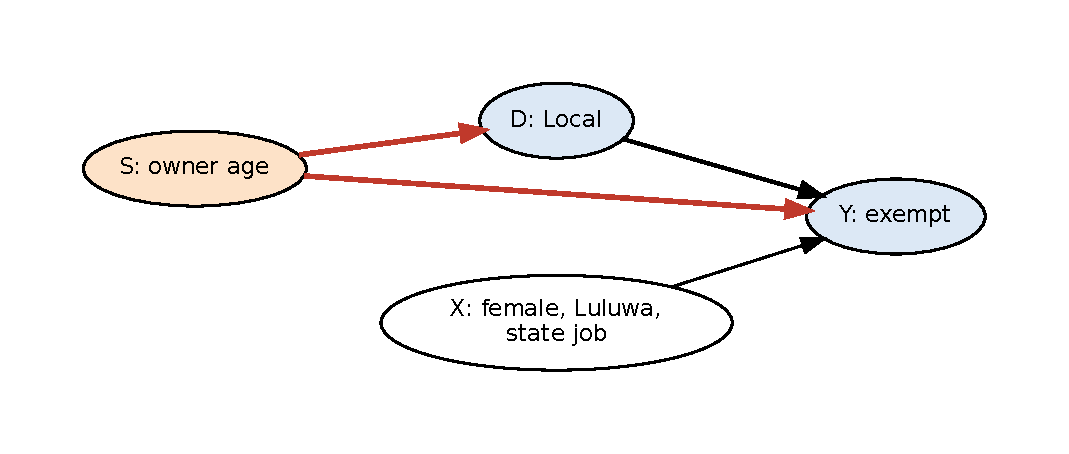
\includegraphics[width=0.55\linewidth]{figure2_dag2.pdf}
\caption{DAG 2. The backdoor path $D \leftarrow S \rightarrow Y$ is in red; $X$ only affects $Y$.}
\end{figure}
\textbf{Step 1, model.} I write DAG 2 as a GML graph (edges $S\to D$, $S\to Y$, $X\to Y$, $D\to Y$) and pass it with the biased sample:
{\footnotesize\begin{verbatim}
model = CausalModel(data=biased, treatment='local', outcome='exempt', graph=gml_graph)
\end{verbatim}}

\textbf{Step 2, identify.} DoWhy prints:
{\footnotesize\begin{verbatim}
Estimand name: backdoor
Estimand expression:  d/d[local] ( E[exempt | owner_age] )
Unconfoundedness: If U->{local} and U->exempt then
  P(exempt|local,owner_age,U) = P(exempt|local,owner_age)
iv: No such variable(s) found!     frontdoor: No such variable(s) found!
\end{verbatim}}
This matches the DAG: the adjustment set is owner age only, since female, Luluwa and state job have no arrow into $D$; no IV or front-door estimand appears, so the graph has no unintended arrows.

\textbf{Step 3, estimate.} \texttt{backdoor.linear\_regression} gives \textbf{0.039}, close to $\taurct=0.031$ and far from $\taunaive=0.200$.

\textbf{Step 4, refute.}
{\footnotesize\begin{verbatim}
Refute: Add a random common cause  Estimated: 0.0386  New effect: 0.0386  p value: 0.98
Refute: Use a subset of data (40%) Estimated: 0.0386  New effect: 0.0365  p value: 0.96
\end{verbatim}}
Adding a made-up common cause leaves the estimate unchanged, and re-estimating on 40\% subsets moves it by only 0.002. Both $p$-values are far above 0.05, so neither test finds a problem with the estimate.

\section{What I learned}
In the biased sample I had to control for owner age only: it is the one variable with arrows into both who collects ($D$) and whether the property is exempted ($Y$), so it opens the backdoor path $D\leftarrow S\rightarrow Y$. Female, Luluwa and state job only affect $Y$; they became unbalanced through their correlation with age, and conditioning on age removes that too. Adjusting for age moves the estimate from 0.200 back to 0.039, close to the experimental 0.031. The assumption I make about everything I did not draw is that no unobserved factor drives both selection and exemption; in a real observational setting the chief's personal tie to the owner would be such a factor, and owner age is partly recorded in age bands, so some confounding could remain. Next, I will estimate heterogeneity with a causal forest, using the endline co-ethnic favouritism question (\texttt{coethnic\_bias\_chief}) to ask whether co-ethnic owners are more likely to be exempted under Local.

\end{document}
